\documentclass[12pt,reqno,intlimits,twoside]{amsart}
\usepackage{amsfonts,amsmath,amsxtra,amsthm,amssymb,latexsym}

\usepackage[dvips]{graphicx}

\usepackage[dvips]{color}

\pagestyle{myheadings}

\evensidemargin=0 cm
\oddsidemargin=0 cm

\textwidth=16 cm
\textheight=21.5 cm

\footskip=1 cm


\def\baselinestretch{1.1}
\parindent= 5mm

\flushbottom
\raggedbottom
\tolerance=1000
\relpenalty=10000
\binoppenalty=10000

\renewcommand{\author}[1]{\begin{center}
{\bfseries{#1}}
\end{center}}

\renewcommand{\title}[1]{
\begin{center}
{\bfseries{#1}}
\end{center}}

\DeclareMathOperator{\erf}{erf}%
\DeclareMathOperator{\erfc}{erfc}%
\DeclareMathOperator{\expL}{expL}%
\DeclareMathOperator{\eeI}{eeI}%
\DeclareMathOperator{\eceI}{eceI}%

\begin{document}

\title{HYDROCYCLONE CALCULATIONS GRAPH}

\author{Tyshkevich Dmitry}

\begin{figure}[!h]
  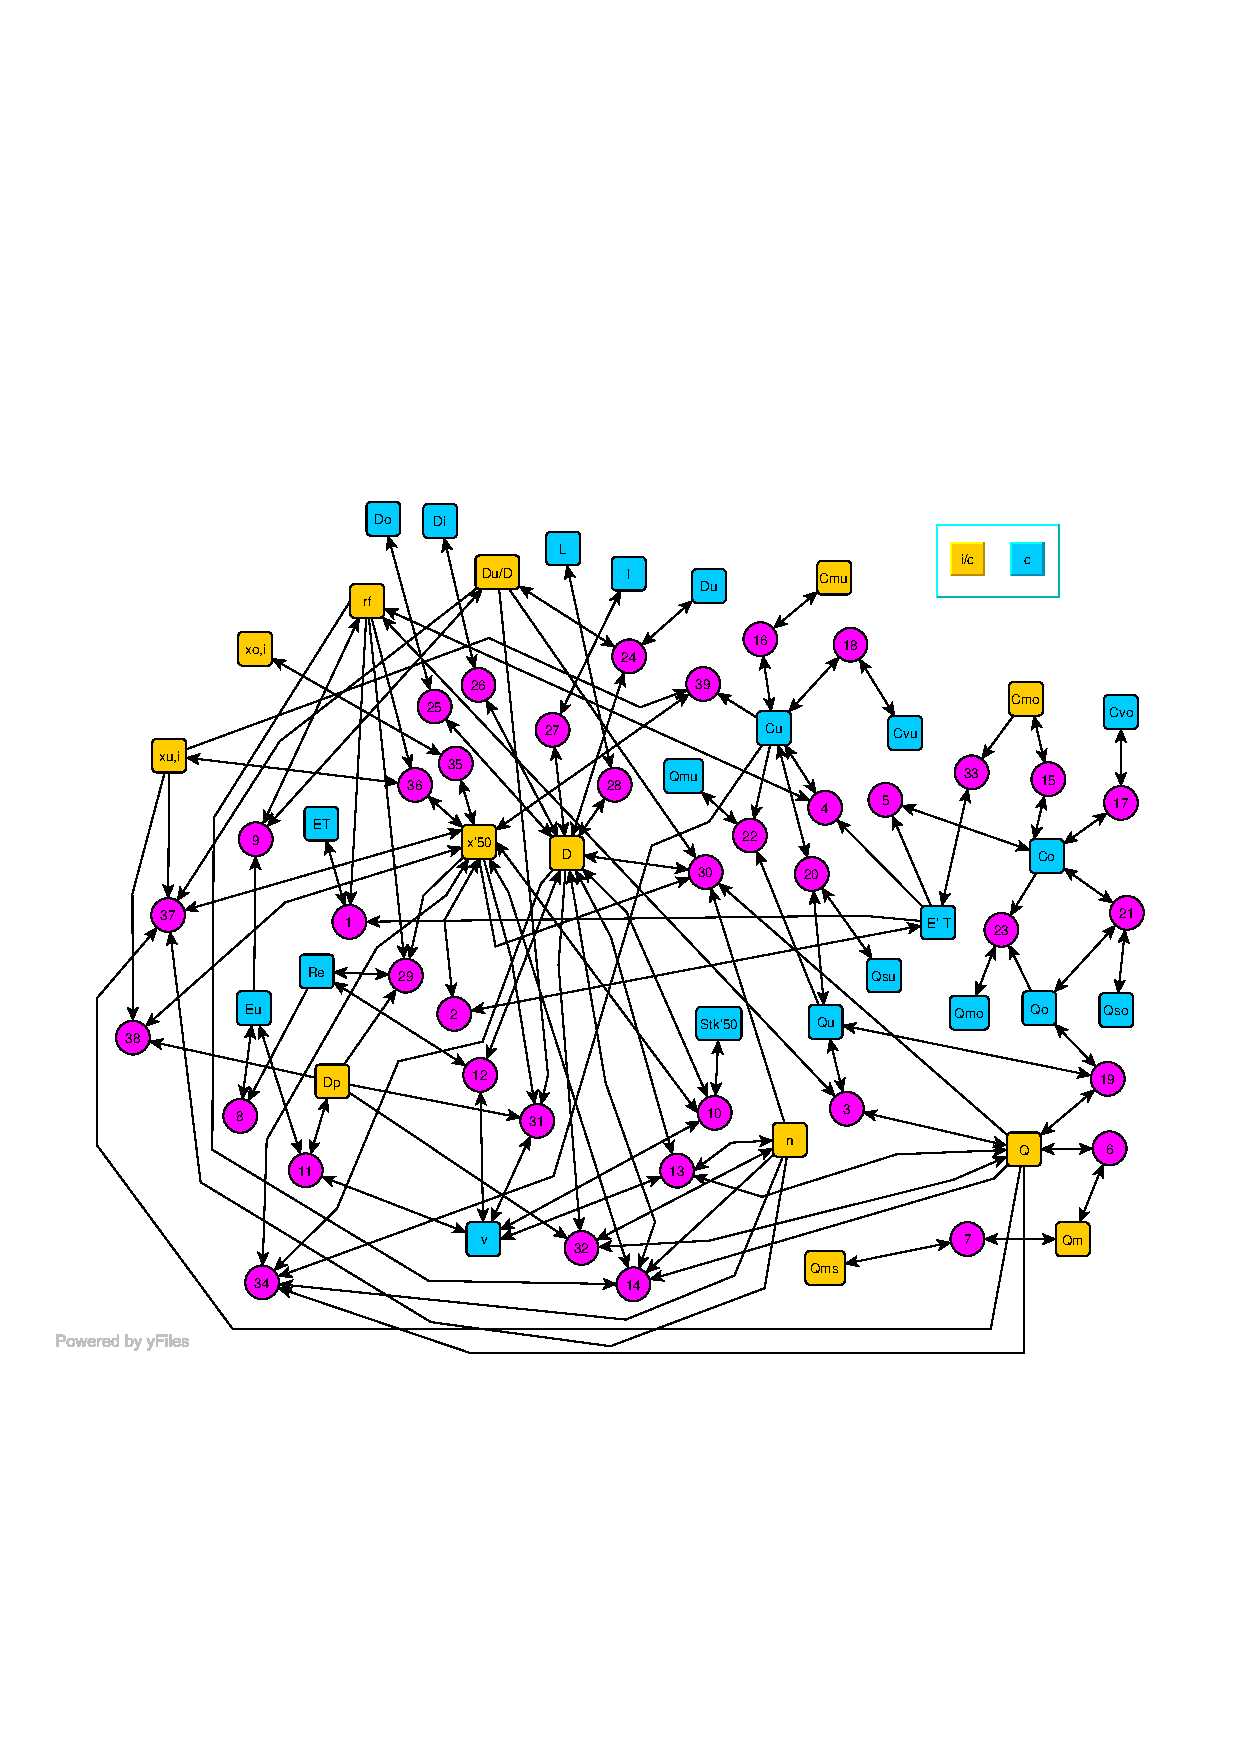
\includegraphics{CalculationGraphHydroCyclone}\\
  \caption{Calculations Graph}\label{FigCalcGraphHydro}
\end{figure}

\newpage

\section{Commentary to the Graph}

Box--shaped verteces correspond to the \textbf{Parameters}. \textcolor{yellow}{Yellow--colored} verteces correspond to
\textbf{input/calculated}  Parameters. \textcolor{blue}{Blue--colored} verteces correspond to only \textbf{calculated} Parameters.

Circle-shaped verteces  correspond to the \textbf{Equations} by wich Paramereters are calculated in the Project.
Inside the circle there is a number corresponding to the equation reference number (see the section~\ref{SectEquations} below).

The absence of an arrow at a Parameter vertex means that this Parameter enters only into the right--hand side of
an equation which sends an (unarrowed) arc to this parameter and only partcipates in calculation of some left--hand side Parameter,
which is to be calculated.
The presence of an an arrow at a Parameter vertex means that this Parameter enters into the left--hand side
(and is to be calculated) of a corresponding equation
which sends an (arrowed) arc to this parameter.

\section{Commentary to the Equations}

The expression  "all terms are derivable" at a \emph{sum} or \emph{product} \emph{equation} means that each Parameter of the equation can enter
into the left--hand side of this general equation (i.e. is derived from the other Parameters and is to be calculated).

By the \textcolor{blue}{blue color} the constant (regarding Calculation Graph in Figure~\ref{FigCalcGraphHydro}) Parameters
(i.e. the Material, Machine Geometry Parameters and constant numbers)
and values calculated by using these constant Parameters are highlighted.

By the \textcolor{green}{green color} auxiliary values, parameters, and functions are highlighted.

By the \textcolor{red}{red color} the new exclusive power-and-fast-implemented functions
\textcolor{red}{$\expL,\;\eeI,\;\eceI$} (see the Sections~\ref{SectExpLin},\:\ref{SectErfExpInt}) are highlighted.

\section{Equations}\label{SectEquations}

\begin{equation}\label{EqERedTrfET} %10
   E_T = (\textcolor{blue}{1} - r_f)E'_T + r_f
\end{equation}

\begin{equation}\label{EqERedTred50} %11
   \left\{
   \begin{array}{l}
      E'_T = \textcolor{blue}{0.5}
              \left(\textcolor{blue}{1} +
                   \erf\left(\dfrac{\textcolor{blue}{\ln(x_g)} - \ln(x'_{50})}
                             {\textcolor{blue}{\sqrt{2}\sqrt{\ln^2(\sigma_g) + \ln^2(\sigma_s)}}}
                       \right)
              \right)  \\
      x'_{50} = \dfrac{\textcolor{blue}{x_g}\strut}%
                      {\exp\left(\erf^{-1}\big(\textcolor{blue}{2}E'_T - \textcolor{blue}{1}\big)
                       \textcolor{blue}{\sqrt{2}\sqrt{\ln^2(\sigma_g) + \ln^2(\sigma_s)}}\right)
                      }
   \end{array}
   \right.
\end{equation}

\begin{equation}\label{EqRfQQu} %15
   r_f Q = Q_u\quad\text{(\emph{product equation}: all terms are derivable )}
\end{equation}

\begin{equation}\label{EqCuRfERedT} %16
   \left\{
   \begin{array}{l}
      c_u = \textcolor{blue}{c}\left(\textcolor{blue}{1} + \dfrac{\textcolor{blue}{1} - r_f}{r_f}E'_T\right)\\
      r_f = \dfrac{\textcolor{blue}{1}\strut}{\textcolor{blue}{1} + \dfrac{\dfrac{c_u}{\textcolor{blue}{c}} - \textcolor{blue}{1}}{E'_T}}
   \end{array}
   \right.
\end{equation}

\begin{equation}\label{EqCoERedT} %17
   c_o = \textcolor{blue}{c}(\textcolor{blue}{1} - E'_T)
\end{equation}

\begin{equation}\label{EqQmQ} %18
   Q_m = \textcolor{blue}{\rho_{sus}} Q\quad\text{(\emph{product equation}: all terms are derivable )}
\end{equation}

\begin{equation}\label{EqQmsQ} %19
   Q_{ms} = \textcolor{blue}{c_m \rho_{sus}} Q\quad\text{(\emph{product equation}: all terms are derivable )}
\end{equation}

\begin{equation}\label{EqEuRe} %21
   Eu = \textcolor{blue}{\beta_1} Re^{\textcolor{blue}{\beta_2}} \textcolor{blue}{\exp(-\beta_3 c_v})
\end{equation}

\begin{equation}\label{EqRfDuDEu} %22
   \left\{
   \begin{array}{l}
      r_f = \textcolor{blue}{\gamma_1} (D_u/D)^{\textcolor{blue}{\gamma_2}} Eu^{-\textcolor{blue}{\gamma_3}}\\
      D_u/D = \left(\dfrac{r_f Eu^{\textcolor{blue}{\gamma_3}}}{\textcolor{blue}{\gamma_1}}\right)^{\textcolor{blue}{\dfrac{1}{\gamma_2}}}
   \end{array}
   \right.
\end{equation}

\begin{equation}\label{EqStkDXRed50v} %23
   \textcolor{blue}{18 \eta}\cdot D\cdot Stk'_{50} = {x'_{50}}^{2}\cdot\textcolor{blue}{(\rho_s - \rho)}\cdot v%
   \quad\text{(\emph{product equation}: all terms are derivable )}
\end{equation}

\begin{equation}\label{EqEuDpv} %24
   \textcolor{blue}{\rho}\cdot Eu\cdot v^2 = \textcolor{blue}{2}\Delta p%
   \quad\text{(\emph{product equation}: all terms are derivable )}
\end{equation}

\begin{equation}\label{EqReDv} %25
   \textcolor{blue}{\eta}\cdot Re = \textcolor{blue}{\rho}\cdot D\cdot v%
   \quad\text{(\emph{product equation}: all terms are derivable )}
\end{equation}

\begin{equation}\label{EqQvDn} %26
   \textcolor{blue}{\pi} D^2\cdot n\cdot v = \textcolor{blue}{4} Q%
   \quad\text{(\emph{product equation}: all terms are derivable )}
\end{equation}

\begin{equation}\label{EqDxRed50} %27
   \left\{
   \begin{array}{l}
      D = \left( \textcolor{blue}{\dfrac{2}{9\pi}}
                 \dfrac{{x'_{50}}^{2}\textcolor{blue}{(\rho_s - \rho)\beta_1}Q%
                        \left(\dfrac{\textcolor{blue}{4\rho}Q}{\textcolor{blue}{\pi\eta}n}\right)^{\textcolor{blue}{\beta_2}}%
                        \exp(\textcolor{blue}{-(\alpha_3 + \beta_3)c_v})}%
                       {\textcolor{blue}{\eta\alpha_1}n\ln^{\textcolor{blue}{\alpha_2}}\left(\dfrac{\textcolor{blue}{1}}{r_f}\right)}
          \right)^{\textcolor{blue}{\dfrac{1}{3 + \beta_2}}}\\
   \phantom{\strut}\\
   x'_{50} = \sqrt{ \strut\textcolor{blue}{\dfrac{9\pi}{2}}
                    \dfrac{\textcolor{blue}{\eta\alpha_1}n\ln^{\textcolor{blue}{\alpha_2}}\left(\dfrac{\textcolor{blue}{1}}{r_f}\right)%
                           D^{\textcolor{blue}{3 + \beta_2}}%
                          }%
                          {\textcolor{blue}{(\rho_s - \rho)\beta_1}Q%
                           \left(\dfrac{\textcolor{blue}{4\rho}Q}{\textcolor{blue}{\pi\eta}n}\right)^{\textcolor{blue}{\beta_2}}%
                           \textcolor{blue}{\exp(-(\alpha_3 + \beta_3)c_v})%
                          }
                  }
   \end{array}
   \right.
\end{equation}

\begin{equation}\label{EqCmoCo} %37.1
   \left\{
   \begin{array}{l}
      c_{mo} = \dfrac{c_o}%
                     {\textcolor{blue}{\rho}%
                     \left(\textcolor{blue}{1} + \dfrac{c_o}{\textcolor{blue}{\rho_s}}%
                     \textcolor{blue}{\left(\dfrac{\rho_s}{\rho} - 1\right)}%
                     \right)%
                     }\\
      \phantom{\strut}\\
      c_o =   \dfrac{1}%
                    {\dfrac{1}{\textcolor{blue}{\rho}c_{mo}} - %
                    \textcolor{blue}{\dfrac{1}{\rho_s}\left(\dfrac{\rho_s}{\rho} - 1\right)}%
                    }
   \end{array}
   \right.
\end{equation}

\begin{equation}\label{EqCmuCu} %37.2
   \left\{
   \begin{array}{l}
      c_{mu} = \dfrac{c_u}%
                     {\textcolor{blue}{\rho}%
                     \left(\textcolor{blue}{1} + \dfrac{c_u}{\textcolor{blue}{\rho_s}}%
                     \textcolor{blue}{\left(\dfrac{\rho_s}{\rho} - 1\right)}%
                     \right)%
                     }\\
      \phantom{\strut}\\
      c_u =   \dfrac{1}%
                    {\dfrac{1}{\textcolor{blue}{\rho}c_{mu}} - %
                    \textcolor{blue}{\dfrac{1}{\rho_s}\left(\dfrac{\rho_s}{\rho} - 1\right)}%
                    }
   \end{array}
   \right.
\end{equation}

\begin{equation}\label{EqCvoCo} %38.1
   \textcolor{blue}{\rho_s} \cdot c_{vo} = c_o%
   \quad\text{(\emph{product equation}: all terms are derivable )}
\end{equation}

\begin{equation}\label{EqCvuCu} %38.2
   \textcolor{blue}{\rho_s} \cdot c_{vu} = c_u%
   \quad\text{(\emph{product equation}: all terms are derivable )}
\end{equation}

\begin{equation}\label{EqQQoQu} %38.3
   Q = Q_o + Q_u%
   \quad\text{(\emph{sum equation}: all terms are derivable )}
\end{equation}

\begin{equation}\label{EqQsuQuCu} %38.4
   Q_{su} = Q_u c_u%
   \quad\text{(\emph{product equation}: all terms are derivable )}
\end{equation}

\begin{equation}\label{EqQsoQoCo} %38.5
   Q_{so} = Q_o c_o%
   \quad\text{(\emph{product equation}: all terms are derivable )}
\end{equation}

\begin{equation}\label{EqQmuQuCu} %38.6
   Q_{mu} = Q_u \left(c_u + (\textcolor{blue}{\rho_s} - c_u)\textcolor{blue}{\dfrac{\rho}{\rho_s}}\right)
\end{equation}

\begin{equation}\label{EqQmoQoCo} %38.7
   Q_{mo} = Q_o \left(c_o + (\textcolor{blue}{\rho_s} - c_o)\textcolor{blue}{\dfrac{\rho}{\rho_s}}\right)
\end{equation}

\begin{equation}\label{EqDuD} %39.1
   D_u = Du/D \cdot D%
   \quad\text{(\emph{product equation}: all terms are derivable )}
\end{equation}

\begin{equation}\label{EqDoD} %39.2
   D_o = \textcolor{blue}{Do/D} \cdot D%
   \quad\text{(\emph{product equation}: all terms are derivable )}
\end{equation}

\begin{equation}\label{EqDiD} %39.3
   D_i = \textcolor{blue}{Di/D} \cdot D%
   \quad\text{(\emph{product equation}: all terms are derivable )}
\end{equation}

\begin{equation}\label{EqlD} %39.4
   l = \textcolor{blue}{l/D} \cdot D%
   \quad\text{(\emph{product equation}: all terms are derivable )}
\end{equation}

\begin{equation}\label{EqLD} %39.5
   L = \textcolor{blue}{L/D} \cdot D%
   \quad\text{(\emph{product equation}: all terms are derivable )}
\end{equation}

\begin{equation}\label{EqReDpRf} %52
   Re = \dfrac{{x'_{50}}^{2}\textcolor{blue}{(\rho_s - \rho)}\Delta p}%
              {\textcolor{blue}{9\eta^2\alpha_1\exp(\alpha_3 c_v)}%
               \ln^{\textcolor{blue}{\alpha_2}}\left(\dfrac{\textcolor{blue}{1}}{r_f}\right)
              }
\end{equation}

\begin{equation}\label{EqDQnxRed50DuD} %67
   \left\{
   \begin{array}{l}
      \text{\emph{We have to solve the transcendental equation:}}\\
      \phantom{\strut}\\
      ?D:\quad%
      \textcolor{blue}{\dfrac{2}{9\pi}}
                 \dfrac{{x'_{50}}^{2}\textcolor{blue}{(\rho_s - \rho)}Q}%
                       {\textcolor{blue}{\eta}nD^3}
      \textcolor{blue}{\beta_1}
      \left(\dfrac{\textcolor{blue}{4\rho} Q}{\textcolor{blue}{\pi\eta}nD}
      \right)^{\textcolor{blue}{\beta_2}}
      \!\!\textcolor{blue}{\exp(-\beta_3 c_v)}=\\
      \phantom{\strut}\\
      \textcolor{blue}{\alpha_1}
      \left( \textcolor{blue}{-\ln(\gamma_1)} -
             \textcolor{blue}{\gamma_2} \ln(Du/D) +
             \textcolor{blue}{\gamma_3}
             \ln\left(\textcolor{blue}{\beta_1}
                     \left(\dfrac{\textcolor{blue}{4\rho} Q}{\textcolor{blue}{\pi\eta}nD}
                     \right)^{\textcolor{blue}{\beta_2}}
      \!\!\textcolor{blue}{\exp(-\beta_3 c_v)}
                \right)
      \right)^{\textcolor{blue}{\alpha_2}}
      \!\!\textcolor{blue}{\exp(\alpha_3 c_v)}\\
      \phantom{\strut}\\
      \text{\emph{The solution can be given by the formula:}}\\
      \phantom{\strut}\\
      D = \left(\exp\big(\textcolor{green}{\mathcal{E}} \cdot \textcolor{green}{\mathcal{F}}\big) \cdot
                \exp\left(\textcolor{red}{\expL^{\infty}_{+}\big(} \textcolor{green}{\mathcal{F}} \cdot
                          \textcolor{green}{\mathcal{G}} \cdot
                                                   \left( \textcolor{green}{\mathcal{A}} \cdot \textcolor{green}{\mathcal{B}}
                                                   \right)^{\textcolor{blue}{\frac{1}{\alpha_2}}}
                                                            \textcolor{red}{\big)}
                    \right)
       \right)^{\textcolor{blue}{\dfrac{-\alpha_2}{3 + \beta_2}}},\quad\text{\emph{where}}\\
      \phantom{\strut}\\
      \textcolor{green}{\mathcal{A}} =
          \textcolor{blue}{\beta_1}
          \left(\dfrac{\textcolor{blue}{4\rho} Q}{\textcolor{blue}{\pi\eta}n}
          \right)^{\textcolor{blue}{\beta_2}}
          \textcolor{blue}{\exp(-\beta_3 c_v)}\\
      \phantom{\strut}\\
      \textcolor{green}{\mathcal{B}} =
      \textcolor{blue}{\dfrac{2}{9\pi}}
                 \dfrac{{x'_{50}}^{2}\textcolor{blue}{(\rho_s - \rho)}Q\,
                        \textcolor{blue}{\exp(-\alpha_3 c_v)}}%
                       {\textcolor{blue}{\eta\alpha_1}n}\\
      \phantom{\strut}\\
      \textcolor{green}{\mathcal{E}} =
      \textcolor{blue}{-\ln(\gamma_1)} -
      \textcolor{blue}{\gamma_2} \ln(Du/D) +
      \textcolor{blue}{\gamma_3} \ln(\textcolor{green}{\mathcal{A}})\\
      \phantom{\strut}\\
      \textcolor{green}{\mathcal{F}} = \textcolor{blue}{\dfrac{3 + \beta_2}{\alpha_2\beta_2\gamma_3}}\\
      \phantom{\strut}\\
      \textcolor{green}{\mathcal{G}} = \exp(-\textcolor{green}{\mathcal{E}} \cdot \textcolor{green}{\mathcal{F}})
   \end{array}
   \right.
\end{equation}

\begin{equation}\label{EqvDuDXRed50Dp} %80
   \left\{
   \begin{array}{l}
      \text{\emph{We have to solve the transcendental equation:}}\\
      \phantom{\strut}\\
      ?v:\quad%
      \dfrac{{x'_{50}}^{2}\textcolor{blue}{(\rho_s - \rho)}\Delta p}%
            {\textcolor{blue}{9\eta^2}%
             \left(\dfrac{\textcolor{blue}{2}\Delta p}%
                         {\textcolor{blue}{\rho\beta_1\exp(-\beta_3 c_v)}v^2}%
             \right)^{\textcolor{blue}{\frac{1}{\beta_2}}}%
            }=\\
      \phantom{\strut}\\
      \textcolor{blue}{\alpha_1}
      \left( \textcolor{blue}{-\ln(\gamma_1)} -
             \textcolor{blue}{\gamma_2} \ln(Du/D) +
             \textcolor{blue}{\gamma_3}
             \ln\left( \dfrac{\textcolor{blue}{2}\Delta p}%
                       {\textcolor{blue}{\rho}v^2}
                \right)
      \right)^{\textcolor{blue}{\alpha_2}}
      \!\!\textcolor{blue}{\exp(\alpha_3 c_v)}\\
      \phantom{\strut}\\
      \text{\emph{The solution can be given by the formula:}}\\
      \phantom{\strut}\\
      v = \left(\textcolor{green}{\mathcal{E}} \cdot
                \exp\left(\textcolor{red}{\expL_-}
                           \textcolor{red}{\big(}
                           %\left(
                          -\textcolor{green}{\mathcal{B}}^{\textcolor{blue}{\frac{1}{\alpha_2}}}
                           \cdot
                           \textcolor{green}{\mathcal{D}} \cdot
                           \textcolor{green}{\mathcal{E}}
                           \textcolor{red}{\big)}
                           %\right)
                    \right)
          \right)^{\textcolor{blue}{\frac{\alpha_2 \beta_2}{2}}},\quad\text{\emph{where}}\\
      \phantom{\strut}\\
     \textcolor{green}{\mathcal{A}} =
     \dfrac{\textcolor{blue}{2}\Delta p}%
     {\textcolor{blue}{\rho}}\\
     \phantom{\strut}\\
     \textcolor{green}{\mathcal{B}} =
     \dfrac{{x'_{50}}^{2}\textcolor{blue}{(\rho_s - \rho)}\Delta p}%
            {\textcolor{blue}{9\eta^2}%
             \left(\dfrac{\textcolor{green}{\mathcal{A}}}%
                         {\textcolor{blue}{\beta_1\exp(-\beta_3 c_v)}}%
             \right)^{\textcolor{blue}{\frac{1}{\beta_2}}}%
             \textcolor{blue}{\alpha_1}\textcolor{blue}{\exp(\alpha_3 c_v)}
            }\\
     \phantom{\strut}\\
     \textcolor{green}{\mathcal{C}} =
     \textcolor{blue}{\alpha_1}
     \big( \textcolor{blue}{-\ln(\gamma_1)} -
            \textcolor{blue}{\gamma_2} \ln(Du/D) +
            \textcolor{blue}{\gamma_3} \ln(\textcolor{green}{\mathcal{A}})
     \big)\\
     \phantom{\strut}\\
     \textcolor{green}{\mathcal{D}} =
     \textcolor{blue}{\dfrac{1}{\alpha_2 \beta_2 \gamma_3}}\\
     \phantom{\strut}\\
     \textcolor{green}{\mathcal{E}} =
     \exp(\textcolor{green}{\mathcal{C}} \cdot  \textcolor{green}{\mathcal{D}})
   \end{array}
   \right.
\end{equation}

\begin{equation}\label{EqQnDpD} %97
   \left\{
   \begin{array}{l}
      Q =
      \left( \dfrac{\textcolor{blue}{\pi^2}\Delta p\,D^4}%
                   {\textcolor{blue}{8\rho \beta_1\exp(-\beta_3 c_v)}%
                    \left(\dfrac{\textcolor{blue}{4\rho}}%
                          {\textcolor{blue}{\pi\eta}D}%
                    \right)^{\textcolor{blue}{\beta_2}}%
                   }
      \right)^{\textcolor{blue}{\frac{1}{2 + \beta_2}}}\!\!\!\!\!\!\!\cdot n\\
      \phantom{\strut}\\
     n =
     \left( \dfrac{\textcolor{blue}{8\rho \beta_1\exp(-\beta_3 c_v)}%
                   \left(\dfrac{\textcolor{blue}{4\rho}}%
                               {\textcolor{blue}{\pi\eta}D}%
                   \right)^{\textcolor{blue}{\beta_2}}%
                  }
                  {\textcolor{blue}{\pi^2}\Delta p\,D^4}%
     \right)^{\textcolor{blue}{\frac{1}{2 + \beta_2}}}\!\!\!\!\!\!\!\cdot Q
   \end{array}
   \right.
\end{equation}

\begin{equation}\label{EqERedTCmo} %x1
   E'_T = 1 - \dfrac{\textcolor{blue}{\rho \rho_s} c_{mo}}%
                    {\textcolor{blue}{c}\big(c_{mo}\textcolor{blue}{(\rho - \rho_s)} +%
                                             \textcolor{blue}{\rho_s}
                                        \big)
                    }
\end{equation}

\begin{equation}\label{EqXRed50} %x2
   \left\{
   \begin{array}{l}
      \text{\emph{We have to solve the transcendental equation:}}\\
      \phantom{\strut}\\
      ?x'_{50}:\quad%
      x'_{50} =
      \left(\dfrac{\textcolor{blue}{9\pi\eta\alpha_1}n%
                   \left(\ln\left(\textcolor{blue}{1} +
                                  \dfrac{\frac{c_u}{\textcolor{blue}{c}} - \textcolor{blue}{1}}%
                                        {\textcolor{blue}{0.5}%
                                         \left(\textcolor{blue}{1} +%
                                               \erf\left(\frac{\textcolor{blue}{\ln(x_g)} - \ln(x'_{50})}%
                                                              {\textcolor{blue}{\sqrt{2}\sqrt{\ln^2(\sigma_g) + \ln^2(\sigma_s)}}}%
                                                   \right)%
                                         \right)%
                                        }%
                            \right)%
                   \right)^{\textcolor{blue}{\alpha_2}}%
                  }
                  {\textcolor{blue}{2(\rho_s - \rho)\beta_1} Q%
                   \left(\dfrac{\textcolor{blue}{4\rho} Q}{\textcolor{blue}{\pi\eta}n}%
                   \right)^{\textcolor{blue}{\beta_2}}%
                   \!\!\textcolor{blue}{\exp\big(-(\alpha_3 + \beta_3) c_v\big)}%
                  }
      \right)^{\textcolor{blue}{\frac{1}{2}}}
      \!\!\cdot D^{\textcolor{blue}{\frac{3 + \beta_2}{2}}}\\
      \phantom{\strut}\\
      \text{\emph{Let's denote}} \\
      \phantom{\strut}\\
      \textcolor{green}{\mathcal{A}} =
      \left(\dfrac{\textcolor{blue}{9\pi\eta\alpha_1\exp\big((\alpha_3 + \beta_3) c_v\big)}n}%
                  {\textcolor{blue}{2(\rho_s - \rho)\beta_1} Q%
                   \left(\dfrac{\textcolor{blue}{4\rho} Q}{\textcolor{blue}{\pi\eta}n}%
                   \right)^{\textcolor{blue}{\beta_2}}%
                  }
      \right)^{\textcolor{blue}{\frac{1}{2}}}
      \!\!\cdot D^{\textcolor{blue}{\frac{3 + \beta_2}{2}}}\\
      \phantom{\strut}\\
      \textcolor{green}{\mathcal{B}} =
      \textcolor{blue}{2}\left(\dfrac{c_u}{\textcolor{blue}{c}} - \textcolor{blue}{1}\right)\qquad\qquad
      \textcolor{green}{\mathcal{E}} =
      \textcolor{blue}{\sqrt{2}\sqrt{\ln^2(\sigma_g) + \ln^2(\sigma_s)}}\\
      \phantom{\strut}\\
      \textcolor{green}{a_1} =
      \dfrac{\ln\left(\frac{xg}{\textcolor{green}{\mathcal{A}}}\right)}{\textcolor{green}{\mathcal{E}}}\qquad\qquad
      \textcolor{green}{a_2} =
      \dfrac{\textcolor{blue}{\alpha_2}}{\textcolor{blue}{2}\textcolor{green}{\mathcal{E}}}\qquad\qquad
      \textcolor{green}{a_3} = \textcolor{green}{\mathcal{B}}\\
      \phantom{\strut}\\
      \text{\emph{Then the above equation is equivalent to the transcendental equation to be solved:}}\\
      \phantom{\strut}\\
      ?\textcolor{green}{x}:\quad%
      \textcolor{green}{x} =
      \textcolor{green}{a_1} -
      \textcolor{green}{a_2}
      \ln\left(\ln\left(\textcolor{blue}{1} +
                        \dfrac{\textcolor{green}{a_3}}{\textcolor{blue}{1} + \erf(\textcolor{green}{x})}
                  \right)
         \right)\\
      \phantom{\strut}\\
      \text{\emph{by using the relations:}}\\
      \phantom{\strut}\\
      x'_{50} = \textcolor{blue}{x_g}\cdot\exp(-\textcolor{green}{x} \cdot \textcolor{green}{\mathcal{E}}),\qquad\qquad
      \textcolor{green}{x} = \dfrac{\textcolor{blue}{\ln(x_g)} - \ln(x'_{50})}{\textcolor{green}{\mathcal{E}}}
      \end{array}
   \right.
\end{equation}

\begin{equation}\label{EqXred50Xoi}  %x3
   \left\{
   \begin{array}{l}
      \text{\emph{We solve the transcendental equation:}}\\
      \phantom{\strut}\\
      \textcolor{red}{\eceI(}\textcolor{green}{b}, \textcolor{green}{z'_{50}}, \textcolor{green}{z_{oi}}
      \textcolor{red}{)} = \textcolor{blue}{2}i\cdot\erfc(\textcolor{green}{a}\cdot \textcolor{green}{z'_{50}})\\
      \phantom{\strut}\\
      \text{\emph{with respect to the }} \textcolor{green}{z'_{50}}
      \text{\emph{ (to find }} x'_{50} \text{\emph{ ) }}
      \text{\emph{ or }}
      \textcolor{green}{z_{oi}}
      \text{\emph{ (to find }} x_{oi} \text{\emph{ ) }}
      \text{\emph{ where}}\\
      \phantom{\strut}\\
      \textcolor{green}{a} =
      \textcolor{blue}{\dfrac{\ln(\sigma_s)}{\sqrt{\ln^2(\sigma_g) + \ln^2(\sigma_s)}}}\qquad\qquad
      \textcolor{green}{b} =
      \textcolor{blue}{\dfrac{\ln(\sigma_g)}{\ln(\sigma_s)}}\\
      \phantom{\strut}\\
      \textcolor{green}{z'_{50}} =
      \dfrac{\textcolor{blue}{\ln(x_g)} - \ln(x'_{50})}{\textcolor{blue}{\sqrt{2}\ln(\sigma_s)}}\qquad\qquad
      \textcolor{green}{z_{oi}} =
      \dfrac{\ln(x_{oi}) - \textcolor{blue}{\ln(x_g)}}{\textcolor{blue}{\sqrt{2}\ln(\sigma_g)}}\\
      \phantom{\strut}\\
      \text{\emph{ Getting calculated }} \textcolor{green}{z'_{50}}
      \text{\emph{ or }} \textcolor{green}{z_{oi}}
      \text{\emph{ we then can calculate }} x'_{50}
      \text{\emph{ or  }} x_{oi}
      \text{\emph{ by the relations: }}\\
      \phantom{\strut}\\
      x'_{50} = \textcolor{blue}{x_g}\cdot\exp(-\textcolor{green}{z'_{50}} \cdot \textcolor{blue}{\sqrt{2}\ln(\sigma_s)})
      \qquad\qquad
      x_{oi} = \textcolor{blue}{x_g}\cdot\exp(\textcolor{green}{z_{oi}} \cdot \textcolor{blue}{\sqrt{2}\ln(\sigma_g)})
      \end{array}
   \right.
\end{equation}

\begin{equation}\label{EqXuiXred50Rf}  %x4
   \left\{
   \begin{array}{l}
      \text{\emph{We solve the transcendental equation:}}\\
      \phantom{\strut}\\
      \textcolor{blue}{1} +
      \erf(\textcolor{green}{z_{ui}}) +
      \textcolor{green}{\widehat{r_f}}\cdot
      \textcolor{red}{\eeI(}\textcolor{green}{b}, \textcolor{green}{z'_{50}}, \textcolor{green}{z_{ui}}
      \textcolor{red}{)} =
      \textcolor{blue}{2}i\cdot
      \big(\textcolor{blue}{1} +
           \textcolor{green}{\widehat{r_f}}\cdot
           \erf(\textcolor{green}{a}\cdot \textcolor{green}{z'_{50}})
      \big)\\
      \phantom{\strut}\\
      \text{\emph{with respect to the }} \textcolor{green}{z'_{50}}
      \text{\emph{ (to find }} x'_{50} \text{\emph{ ) }}
      \text{\emph{ or }}
      \textcolor{green}{z_{ui}}
      \text{\emph{ (to find }} x_{ui} \text{\emph{ ) }}
      \text{\emph{ where}}\\
      \phantom{\strut}\\
      \textcolor{green}{a} =
      \textcolor{blue}{\dfrac{\ln(\sigma_s)}{\sqrt{\ln^2(\sigma_g) + \ln^2(\sigma_s)}}}\qquad\qquad
      \textcolor{green}{b} =
      \textcolor{blue}{\dfrac{\ln(\sigma_g)}{\ln(\sigma_s)}}\qquad\qquad
      \textcolor{green}{\widehat{r_f}} =
      \dfrac{\textcolor{blue}{1} - r_f}{\textcolor{blue}{1} + r_f}\\
      \phantom{\strut}\\
      \textcolor{green}{z'_{50}} =
      \dfrac{\textcolor{blue}{\ln(x_g)} - \ln(x'_{50})}{\textcolor{blue}{\sqrt{2}\ln(\sigma_s)}}\qquad\qquad
      \textcolor{green}{z_{ui}} =
      \dfrac{\ln(x_{ui}) - \textcolor{blue}{\ln(x_g)}}{\textcolor{blue}{\sqrt{2}\ln(\sigma_g)}}\\
      \phantom{\strut}\\
      \text{\emph{ Getting calculated }} \textcolor{green}{z'_{50}}
      \text{\emph{ or }} \textcolor{green}{z_{ui}}
      \text{\emph{ we then can calculate }} x'_{50}
      \text{\emph{ or  }} x_{ui}
      \text{\emph{ by the relations: }}\\
      \phantom{\strut}\\
      x'_{50} = \textcolor{blue}{x_g}\cdot\exp(-\textcolor{green}{z'_{50}} \cdot \textcolor{blue}{\sqrt{2}\ln(\sigma_s)})
      \qquad\qquad
      x_{ui} = \textcolor{blue}{x_g}\cdot\exp(\textcolor{green}{z_{ui}} \cdot \textcolor{blue}{\sqrt{2}\ln(\sigma_g)})
      \end{array}
   \right.
\end{equation}

\begin{equation}\label{EqXred50XuiDuDQn}  %x5
   \left\{
   \begin{array}{l}
      \text{\emph{We solve the transcendental equation:}}\\
      \phantom{\strut}\\
      ?\textcolor{green}{z'_{50}}:\quad%
      \textcolor{blue}{1} +
      \erf(\textcolor{green}{z_{ui}}) +
      \textcolor{green}{\widehat{R_f}(z'_{50})}\cdot
      \textcolor{red}{\eeI(}\textcolor{green}{b}, \textcolor{green}{z'_{50}}, \textcolor{green}{z_{ui}}
      \textcolor{red}{)} =
      \textcolor{blue}{2}i\cdot
      \big(\textcolor{blue}{1} +
           \textcolor{green}{\widehat{R_f}(z'_{50})}\cdot
           \erf(\textcolor{green}{a}\cdot \textcolor{green}{z'_{50}})
      \big),\\
      \phantom{\strut}\\
      \text{\emph{ where}}\\
      \phantom{\strut}\\
      \textcolor{green}{a} =
      \textcolor{blue}{\dfrac{\ln(\sigma_s)}{\sqrt{\ln^2(\sigma_g) + \ln^2(\sigma_s)}}}\qquad\qquad
      \textcolor{green}{b} =
      \textcolor{blue}{\dfrac{\ln(\sigma_g)}{\ln(\sigma_s)}}\qquad\qquad
      \textcolor{green}{z_{ui}} =
      \dfrac{\ln(x_{ui}) - \textcolor{blue}{\ln(x_g)}}{\textcolor{blue}{\sqrt{2}\ln(\sigma_g)}}\\
      \phantom{\strut}\\
      \textcolor{green}{\widehat{R_f}(}\zeta\textcolor{green}{)} =
      \dfrac{\textcolor{blue}{1} - \textcolor{green}{R_f(}\zeta\textcolor{green}{)}}%
            {\textcolor{blue}{1} + \textcolor{green}{R_f(}\zeta\textcolor{green}{)}}
      \qquad\qquad
      \textcolor{green}{R_f(}\zeta\textcolor{green}{)} =
      \textcolor{red}{\expL_+^{\infty}\bigg(}
      \textcolor{blue}{\dfrac{3 + \beta_2}{\alpha_2\beta_2\gamma_3}}\cdot
      \textcolor{green}{\mathfrak{a}(}\zeta\textcolor{green}{)}^%
      {\textcolor{blue}{-\frac{3 + \beta_2}{\alpha_2\beta_2}}}
      \textcolor{red}{\bigg)}\\
      \phantom{\strut}\\
      \textcolor{green}{\mathfrak{a}(}\zeta\textcolor{green}{)} =
      \textcolor{green}{\mathcal{A}} \cdot
      \big(\textcolor{blue}{x_g}\cdot\exp(-\zeta \cdot \textcolor{blue}{\sqrt{2}\ln(\sigma_s)})
      \big)^%
      {\textcolor{blue}{-\frac{2\beta_2}{3 + \beta_2}}}\\
      \phantom{\strut}\\
      \textcolor{green}{\mathcal{A}} =
      \left( \textcolor{blue}{\gamma_1}
             (D_u/D)^{\textcolor{blue}{\gamma_2}}
      \right)^{\textcolor{blue}{-\frac{1}{\gamma_3}}}
      \textcolor{blue}{\beta_1}
      \left(\textcolor{green}{\mathcal{B}} \cdot
            \left(\textcolor{blue}{\big(\frac{\pi}{12}\big)^2
                                   \frac{\beta_1}{2\alpha_1}
                                   \big(\frac{\rho_s}{\rho} - 1\big)
                                   \text{e}^{-(\alpha_1 + \beta_3) c_v}\cdot
                                   \textcolor{green}{\mathcal{B}}^{\textcolor{blue}{\beta_2 + 1}}
                                  }
            \right)^{\textcolor{blue}{-\frac{1}{3 + \beta_2}}}
      \right)^{\textcolor{blue}{\beta_2}} \!\!\textcolor{blue}{\text{e}^{-\beta_3 c_v}}\\
      \phantom{\strut}\\
      \textcolor{green}{\mathcal{B}} =
      \dfrac{\textcolor{blue}{\rho} Q}{\textcolor{blue}{\eta} n}\\
      \phantom{\strut}\\
      \text{\emph{ Getting calculated }} \textcolor{green}{z'_{50}}
      \text{\emph{ we then calculate }} x'_{50}
      \text{\emph{ by the relation: }}\\
      \phantom{\strut}\\
      x'_{50} = \textcolor{blue}{x_g}\cdot\exp(-\textcolor{green}{z'_{50}} \cdot \textcolor{blue}{\sqrt{2}\ln(\sigma_s)})
      \end{array}
   \right.
\end{equation}

\begin{equation}\label{EqXred50XuiDpDuD}  %x6
   \left\{
   \begin{array}{l}
      \text{\emph{We solve the transcendental equation:}}\\
      \phantom{\strut}\\
      ?\textcolor{green}{z'_{50}}:\quad%
      \textcolor{blue}{1} +
      \erf(\textcolor{green}{z_{ui}}) +
      \textcolor{green}{\widehat{R_f}(z'_{50})}\cdot
      \textcolor{red}{\eeI(}\textcolor{green}{b}, \textcolor{green}{z'_{50}}, \textcolor{green}{z_{ui}}
      \textcolor{red}{)} =
      \textcolor{blue}{2}i\cdot
      \big(\textcolor{blue}{1} +
           \textcolor{green}{\widehat{R_f}(z'_{50})}\cdot
           \erf(\textcolor{green}{a}\cdot \textcolor{green}{z'_{50}})
      \big),\\
      \phantom{\strut}\\
      \text{\emph{ where}}\\
      \phantom{\strut}\\
      \textcolor{green}{a} =
      \textcolor{blue}{\dfrac{\ln(\sigma_s)}{\sqrt{\ln^2(\sigma_g) + \ln^2(\sigma_s)}}}\qquad\qquad
      \textcolor{green}{b} =
      \textcolor{blue}{\dfrac{\ln(\sigma_g)}{\ln(\sigma_s)}}\qquad\qquad
      \textcolor{green}{z_{ui}} =
      \dfrac{\ln(x_{ui}) - \textcolor{blue}{\ln(x_g)}}{\textcolor{blue}{\sqrt{2}\ln(\sigma_g)}}\\
      \phantom{\strut}\\
      \textcolor{green}{\widehat{R_f}(}\zeta\textcolor{green}{)} =
      \dfrac{\textcolor{blue}{1} - \textcolor{green}{R_f(}\zeta\textcolor{green}{)}}%
            {\textcolor{blue}{1} + \textcolor{green}{R_f(}\zeta\textcolor{green}{)}}
      \qquad\qquad
      \textcolor{green}{R_f(}\zeta\textcolor{green}{)} =
      \textcolor{red}{\expL_-\bigg(}
      \textcolor{blue}{\dfrac{-1}{\alpha_2\beta_2\gamma_3}}\cdot
      \textcolor{green}{\mathfrak{a}(}\zeta\textcolor{green}{)}^%
      {\textcolor{blue}{\frac{1}{\alpha_2\beta_2}}}
      \textcolor{red}{\bigg)}\\
      \phantom{\strut}\\
      \textcolor{green}{\mathfrak{a}(}\zeta\textcolor{green}{)} =
      \textcolor{green}{\mathcal{A}} \cdot
      \big(\textcolor{blue}{x_g}\cdot\exp(-\zeta \cdot \textcolor{blue}{\sqrt{2}\ln(\sigma_s)})
      \big)^%
      {\textcolor{blue}{2\beta_2}}\\
      \phantom{\strut}\\
      \textcolor{green}{\mathcal{A}} =
      \left( \textcolor{blue}{\gamma_1}
             (D_u/D)^{\textcolor{blue}{\gamma_2}}
      \right)^{\textcolor{blue}{-\frac{1}{\gamma_3}}}
      \textcolor{blue}{\beta_1}
      \left(\dfrac{\textcolor{blue}{(\rho_s - \rho)\text{e}^{-\alpha_3 c_v}}\,\Delta p}%
                  {\textcolor{blue}{9\eta^2\alpha_1}}
      \right)^{\textcolor{blue}{\beta_2}} \!\!\textcolor{blue}{\text{e}^{-\beta_3 c_v}}\\
      \phantom{\strut}\\
      \text{\emph{ Getting calculated }} \textcolor{green}{z'_{50}}
      \text{\emph{ we then calculate }} x'_{50}
      \text{\emph{ by the relation: }}\\
      \phantom{\strut}\\
      x'_{50} = \textcolor{blue}{x_g}\cdot\exp(-\textcolor{green}{z'_{50}} \cdot \textcolor{blue}{\sqrt{2}\ln(\sigma_s)})
      \end{array}
   \right.
\end{equation}

\begin{equation}\label{EqXred50XuiCuC}  %x7
   \left\{
   \begin{array}{l}
      \text{\emph{We solve the transcendental equation:}}\\
      \phantom{\strut}\\
      ?\textcolor{green}{z'_{50}}:\quad%
      \textcolor{blue}{1} +
      \erf(\textcolor{green}{z_{ui}}) +
      \textcolor{green}{\widehat{R_f}(z'_{50})}\cdot
      \textcolor{red}{\eeI(}\textcolor{green}{b}, \textcolor{green}{z'_{50}}, \textcolor{green}{z_{ui}}
      \textcolor{red}{)} =
      \textcolor{blue}{2}i\cdot
      \big(\textcolor{blue}{1} +
           \textcolor{green}{\widehat{R_f}(z'_{50})}\cdot
           \erf(\textcolor{green}{a}\cdot \textcolor{green}{z'_{50}})
      \big),\\
      \phantom{\strut}\\
      \text{\emph{ where}}\\
      \phantom{\strut}\\
      \textcolor{green}{a} =
      \textcolor{blue}{\dfrac{\ln(\sigma_s)}{\sqrt{\ln^2(\sigma_g) + \ln^2(\sigma_s)}}}\qquad\qquad
      \textcolor{green}{b} =
      \textcolor{blue}{\dfrac{\ln(\sigma_g)}{\ln(\sigma_s)}}\qquad\qquad
      \textcolor{green}{z_{ui}} =
      \dfrac{\ln(x_{ui}) - \textcolor{blue}{\ln(x_g)}}{\textcolor{blue}{\sqrt{2}\ln(\sigma_g)}}\\
      \phantom{\strut}\\
      \textcolor{green}{\widehat{R_f}(}\zeta\textcolor{green}{)} =
      \dfrac{\textcolor{blue}{1} - \textcolor{green}{R_f(}\zeta\textcolor{green}{)}}%
            {\textcolor{blue}{1} + \textcolor{green}{R_f(}\zeta\textcolor{green}{)}}
      \qquad\qquad
      \textcolor{green}{R_f(}\zeta\textcolor{green}{)} =
      \dfrac{\textcolor{blue}{1}}%
            {\textcolor{blue}{1} +
             \dfrac{\textcolor{blue}{2}\Big(\dfrac{c_u}{\textcolor{blue}{c}} - \textcolor{blue}{1}\Big)}%
                   {\textcolor{blue}{1} + \erf(\textcolor{green}{a} \cdot \zeta)}%
            }\\
      \phantom{\strut}\\
      \text{\emph{ Getting calculated }} \textcolor{green}{z'_{50}}
      \text{\emph{ we then calculate }} x'_{50}
      \text{\emph{ by the relation: }}\\
      \phantom{\strut}\\
      x'_{50} = \textcolor{blue}{x_g}\cdot\exp(-\textcolor{green}{z'_{50}} \cdot \textcolor{blue}{\sqrt{2}\ln(\sigma_s)})
      \end{array}
   \right.
\end{equation}

\section{The functions $\expL_+^{\infty},\ \expL_+^{0}, \ \expL_-$}\label{SectExpLin}

The transcendental equation
\begin{equation}\label{EqZxExpz}
   z = x\exp(z)
\end{equation}
with respect to $z$ given $x$ has a \emph{unique} solution if $x < 0$ and \emph{exactly two} solutions if
\begin{equation*}
   0 < x < \exp(-1) \approx 0.367879441171442321595524
\end{equation*}
If $x = \exp(-1)$ then \eqref{EqZxExpz}  has a unique solution $z = 1$; if $x > \exp(-1)$
then \eqref{EqZxExpz}  \emph{has no} solution.

So for the domain $(0, \exp(-1)]$ we have two branches of $z(x)$: the first one,  $\expL_+^{\infty}$, for which
$$
   \text{if}\;x\rightarrow0\quad\text{then}\;z\rightarrow\infty
$$
and the second one, $\expL_+^{0}$, for which
$$
   \text{if}\;x\rightarrow0\quad\text{then}\;z\rightarrow0.
$$
By $\expL_-$ we denote the function $0 > x \mapsto z(x)$.

\section{The functions $\eeI,\ \eceI$}\label{SectErfExpInt}
We introduce the function
\begin{equation}\label{EqErfExpInt}
   \eeI(a, b, x) =
   \frac{2}{\sqrt{\pi}}
   \int_{-\infty}^{x}\!\erf(at + b)\exp(-t^2)dt
\end{equation}

This function satisfies the following notable equalities
\begin{align*}
  &
  \eeI(a, b, x) =
  \left\{
    \begin{array}{ll}
       \erf(ax + b)\erf(x) - 1 - \eeI\big(\frac{1}{a}, -\frac{b}{a}, ax + b\big), &         a > 0 \\
       \erf(b)\big(1 + \erf(x)\big),  &  a = 0 \\
       \erf(ax + b)\erf(x) + 1 + \eeI\big(-\frac{1}{a}, -\frac{b}{a}, -ax - b\big),   &      a < 0
    \end{array}
  \right.\\
  &
  \eeI(-a, -b, x) = -\eeI(a, b, x)
\end{align*}

Some plots regarding $\eeI$ are shown in Figures~\ref{FigErfExpInt_b},\:\ref{FigErfExpInt_x}.

Also we introduce the function
\begin{equation}\label{EqErfcExpInt}
   \eceI(a, b, x) =
   \frac{2}{\sqrt{\pi}}
   \int_{-\infty}^{x}\!\erfc(at + b)\exp(-t^2)dt =
   1 + \erf(x) + \eeI(a,b,x)
\end{equation}

\section{The Feed Functions and their connection with $\eeI,\ \eceI$}

The \textbf{Feed Functions} are defined by the following formulae
(by the red color the main argument is highlighted; by the blue color the constant Parameters
correspondigly to the equations in the Section~\ref{SectEquations} are highlighted;
by the green color auxiliary parameters are highlighted):
\begin{align*}
   & F_o(r_f, x'_{50}, \textcolor{red}{x}) =
     \dfrac{1}{\textcolor{blue}{1} - E_T(r_f, x'_{50})}
     \int_{0}^{\textcolor{red}{x}}\big(\textcolor{blue}{1} - G(r_f, x'_{50}, t)\big)\dot{F}(t)dt\\
   & F_u(r_f, x'_{50}, \textcolor{red}{x}) =
     \dfrac{1}{E_T(r_f, x'_{50})}
     \int_{0}^{\textcolor{red}{x}}G(r_f, x'_{50}, t)\dot{F}(t)dt
\end{align*}
($\dot{F}(t)$ is a derivative of $F(t)$, $\frac{dF}{dt}$) where
\begin{align*}
   & E_T(r_f, x'_{50}) = (\textcolor{blue}{1} - r_f)E'_T(x'_{50}) + r_f;\\
   & E'_T(x'_{50}) = \textcolor{blue}{0.5}
                     \left(\textcolor{blue}{1} +
                           \erf\left(\dfrac{\textcolor{blue}{\ln(x_g)} - \ln(x'_{50})}
                                           {\textcolor{blue}{\sqrt{2}\sqrt{\ln^2(\sigma_g) + \ln^2(\sigma_s)}}}
                                \right)
                     \right);\\
   & F(\textcolor{red}{x}) =
     \textcolor{blue}{0.5}
     \left(\textcolor{blue}{1} +
           \erf\left(\dfrac{\ln(\textcolor{red}{x}) - \textcolor{blue}{\ln(x_g)}}
                           {\textcolor{blue}{\sqrt{2}\ln(\sigma_g)}}
               \right)
     \right);\\
   & G(r_f, x'_{50}, \textcolor{red}{x}) =
     (\textcolor{blue}{1} - r_f)G'(x'_{50}, \textcolor{red}{x}) + r_f;\\
   & G'(x'_{50}, \textcolor{red}{x}) =
     \textcolor{blue}{0.5}
     \left(\textcolor{blue}{1} +
           \erf\left(\dfrac{\ln(\textcolor{red}{x}) - \ln(x'_{50})}
                           {\textcolor{blue}{\sqrt{2}\ln(\sigma_s)}}
               \right)
     \right);
\end{align*}

The following relations hold:
\begin{align*}
   & (1 - E_T) F_o(\textcolor{red}{x}) + E_T F_u(\textcolor{red}{x})= F(\textcolor{red}{x});\\
   & F_o(r_f, x'_{50}, \textcolor{red}{x}) =
     \textcolor{blue}{0.5}\,
     \dfrac{\eceI(\textcolor{green}{b}, \textcolor{green}{z'_{50}}, \textcolor{green}{z})}%
           {\erfc(\textcolor{green}{a}\cdot \textcolor{green}{z'_{50}})};\\
   & F_u(r_f, x'_{50}, \textcolor{red}{x}) =
     \textcolor{blue}{0.5}\,
     \dfrac{\textcolor{blue}{1} +
            \erf(\textcolor{green}{z}) +
            \textcolor{green}{\widehat{r_f}}\cdot
            \eeI(\textcolor{green}{b}, \textcolor{green}{z'_{50}}, \textcolor{green}{z})
           }%
           {\textcolor{blue}{1} +
            \textcolor{green}{\widehat{r_f}}\cdot
            \erf(\textcolor{green}{a}\cdot \textcolor{green}{z'_{50}})
           }
\end{align*}
where
\begin{align*}
  &
  \textcolor{green}{a} =
  \textcolor{blue}{\dfrac{\ln(\sigma_s)}{\sqrt{\ln^2(\sigma_g) + \ln^2(\sigma_s)}}};\quad
  \textcolor{green}{b} =
  \textcolor{blue}{\dfrac{\ln(\sigma_g)}{\ln(\sigma_s)}};\quad
  \textcolor{green}{\widehat{r_f}} =
  \dfrac{\textcolor{blue}{1} - r_f}{\textcolor{blue}{1} + r_f}\\
  &
  \textcolor{green}{z} =
  \dfrac{\ln(\textcolor{red}{x}) - \textcolor{blue}{\ln(x_g)}}{\textcolor{blue}{\sqrt{2}\ln(\sigma_g)}};\quad
  \textcolor{green}{z'_{50}} =
  \dfrac{\textcolor{blue}{\ln(x_g)} - \ln(x'_{50})}{\textcolor{blue}{\sqrt{2}\ln(\sigma_s)}}
\end{align*}


\newpage

\begin{figure}[!h]
  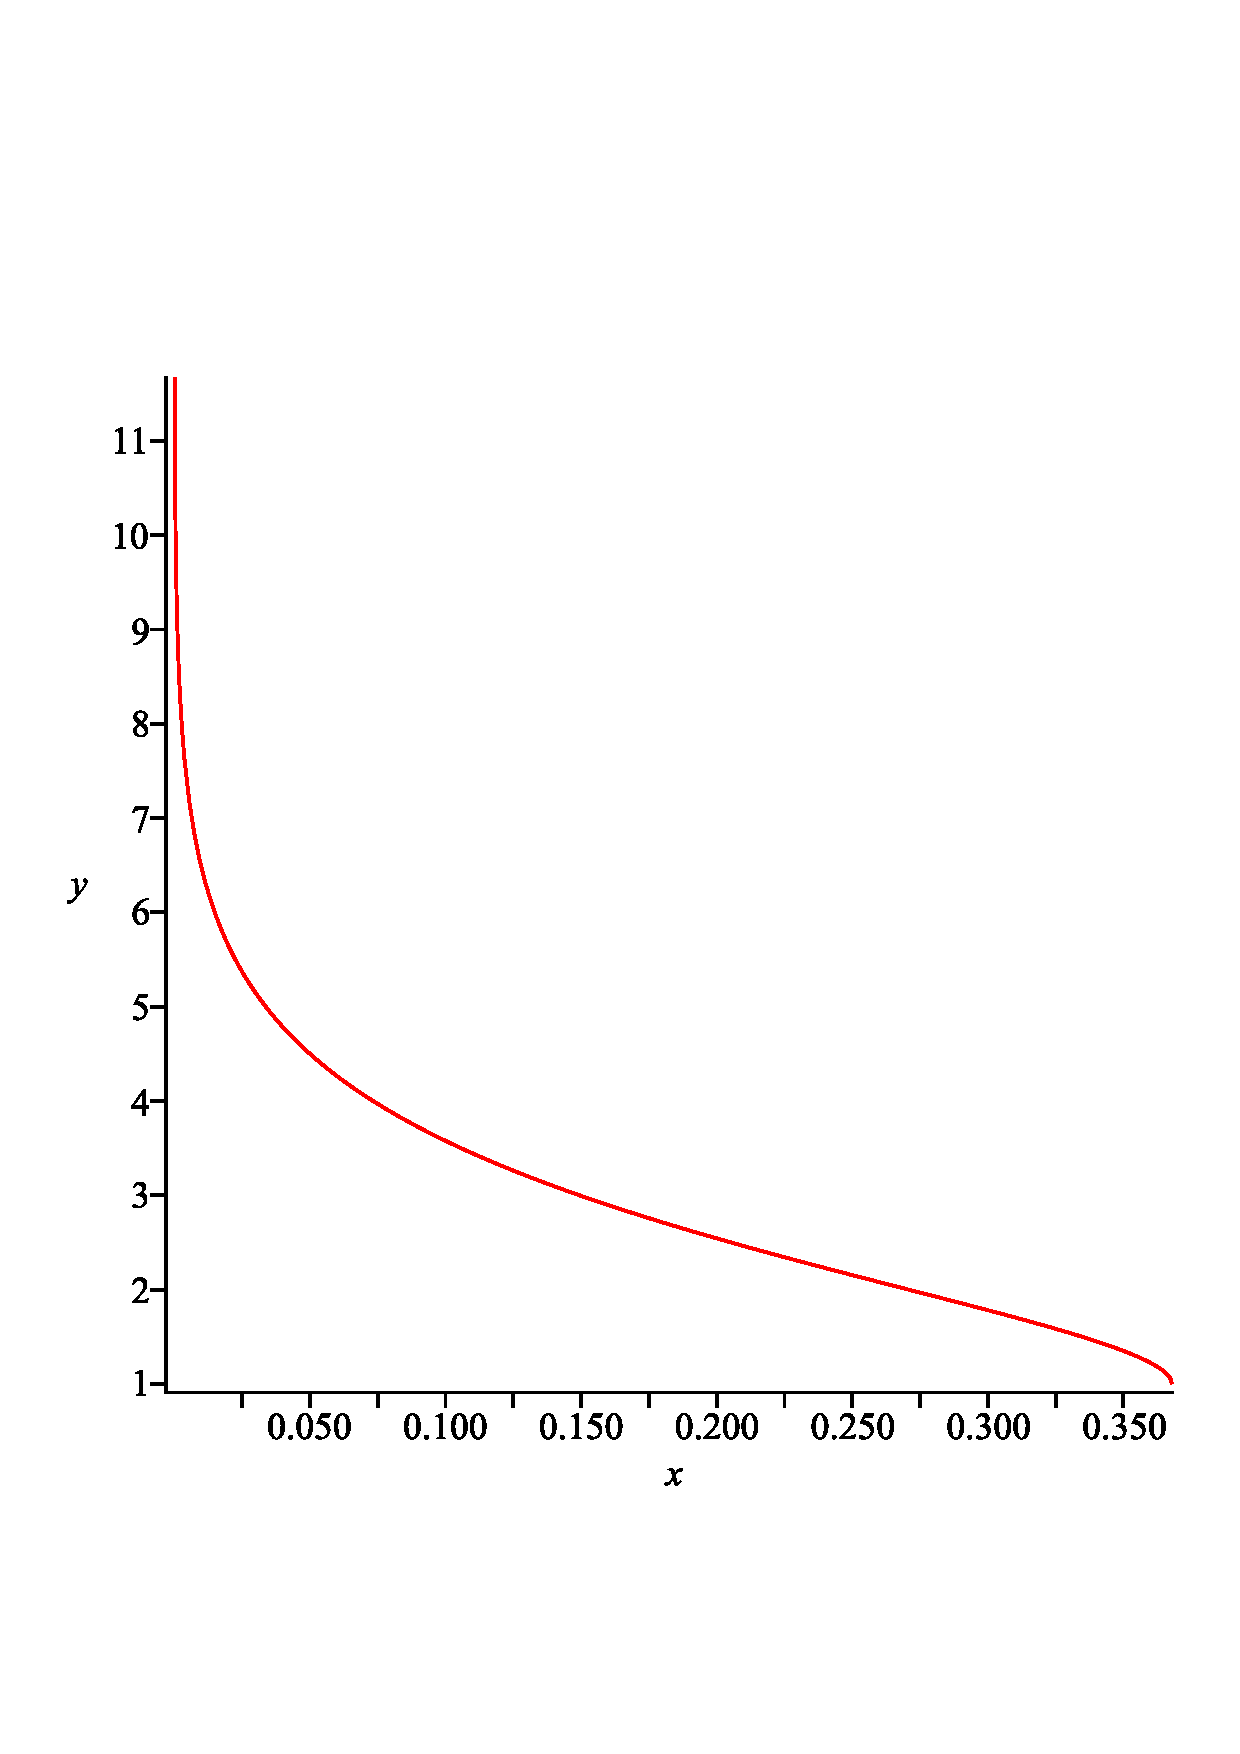
\includegraphics{ExpLinPosInfinity}\\
  \caption{$y=\textcolor{red}{\expL_+^{\infty}(}x\textcolor{red}{)}$}\label{FigExpLinPosInfinity}
\end{figure}

\newpage

\begin{figure}[!h]
  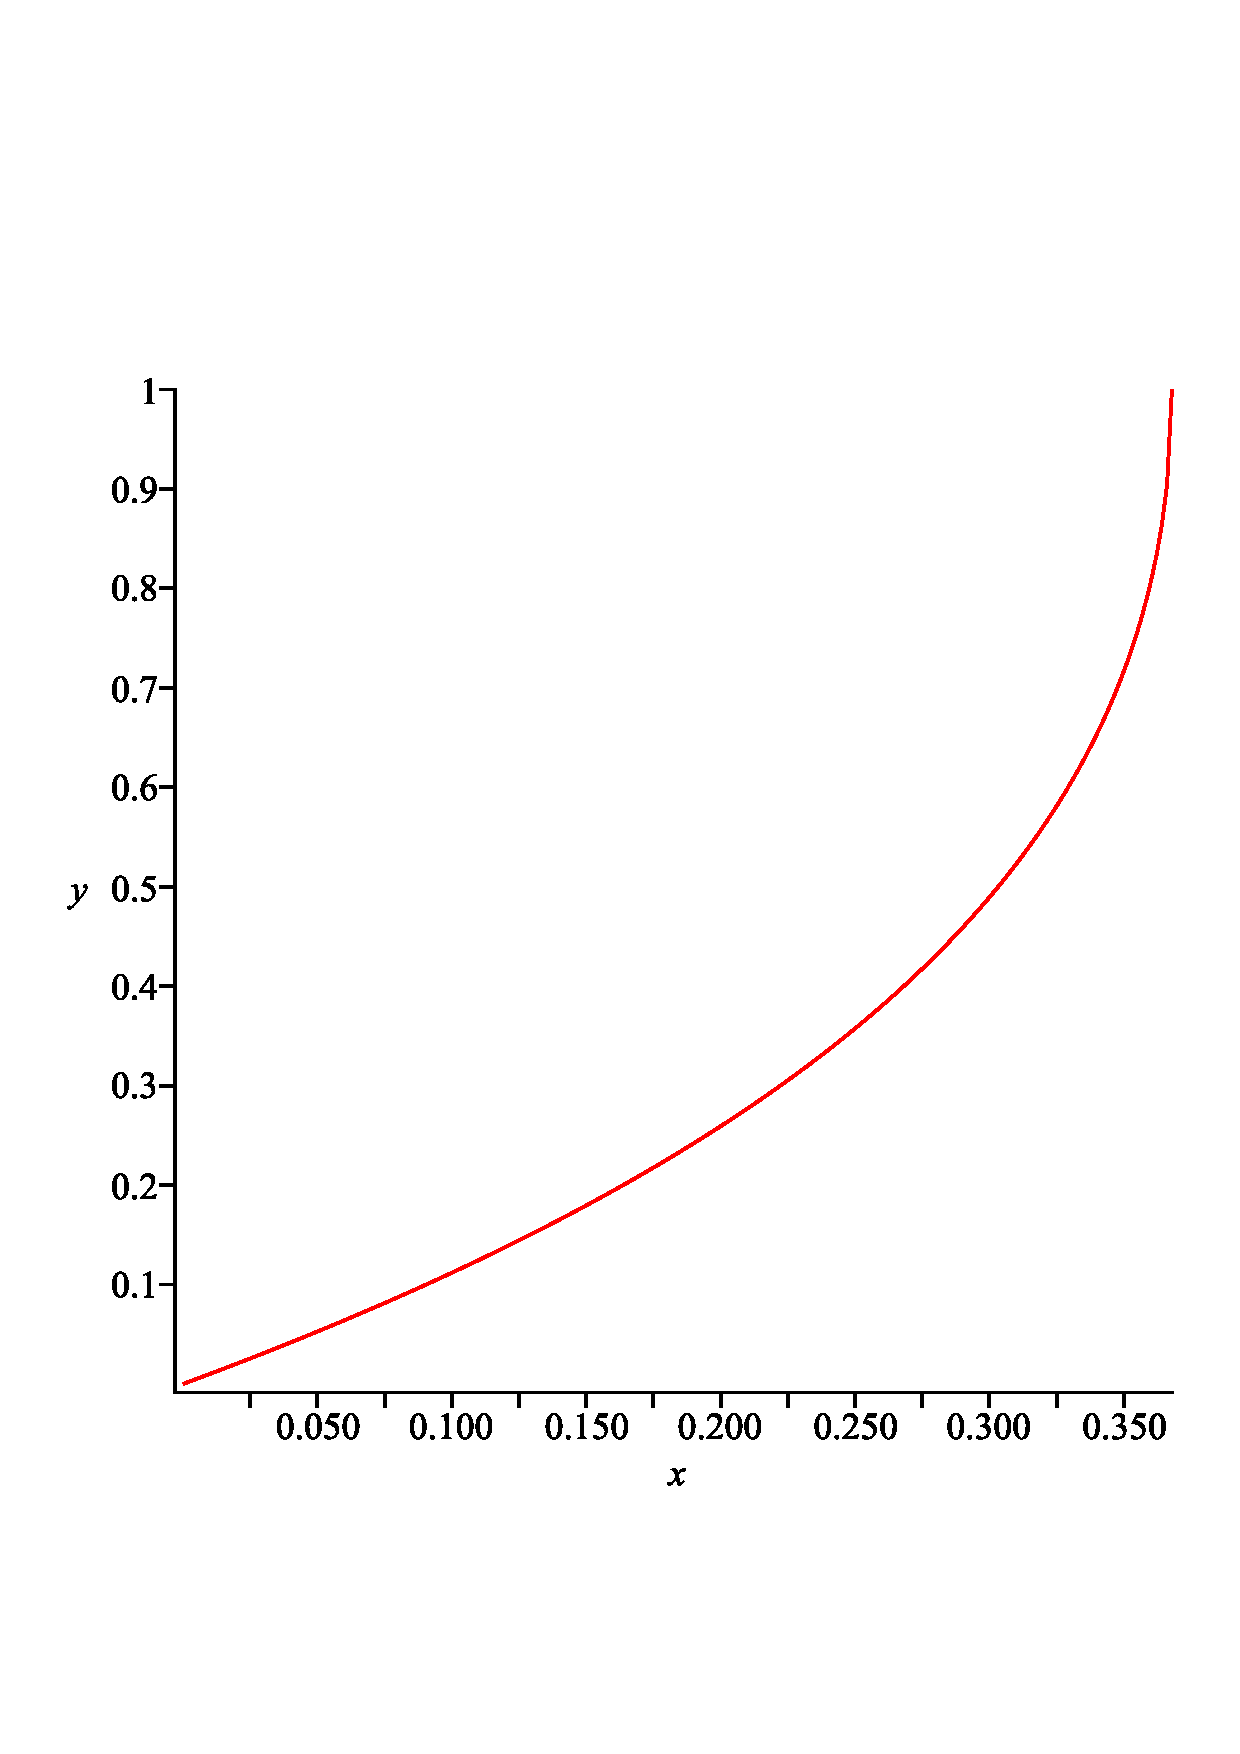
\includegraphics{ExpLinPosZero}\\
  \caption{$y=\textcolor{red}{\expL_+^{0}(}x\textcolor{red}{)}$}\label{FigExpLinPosZero}
\end{figure}

\newpage

\begin{figure}[!h]
  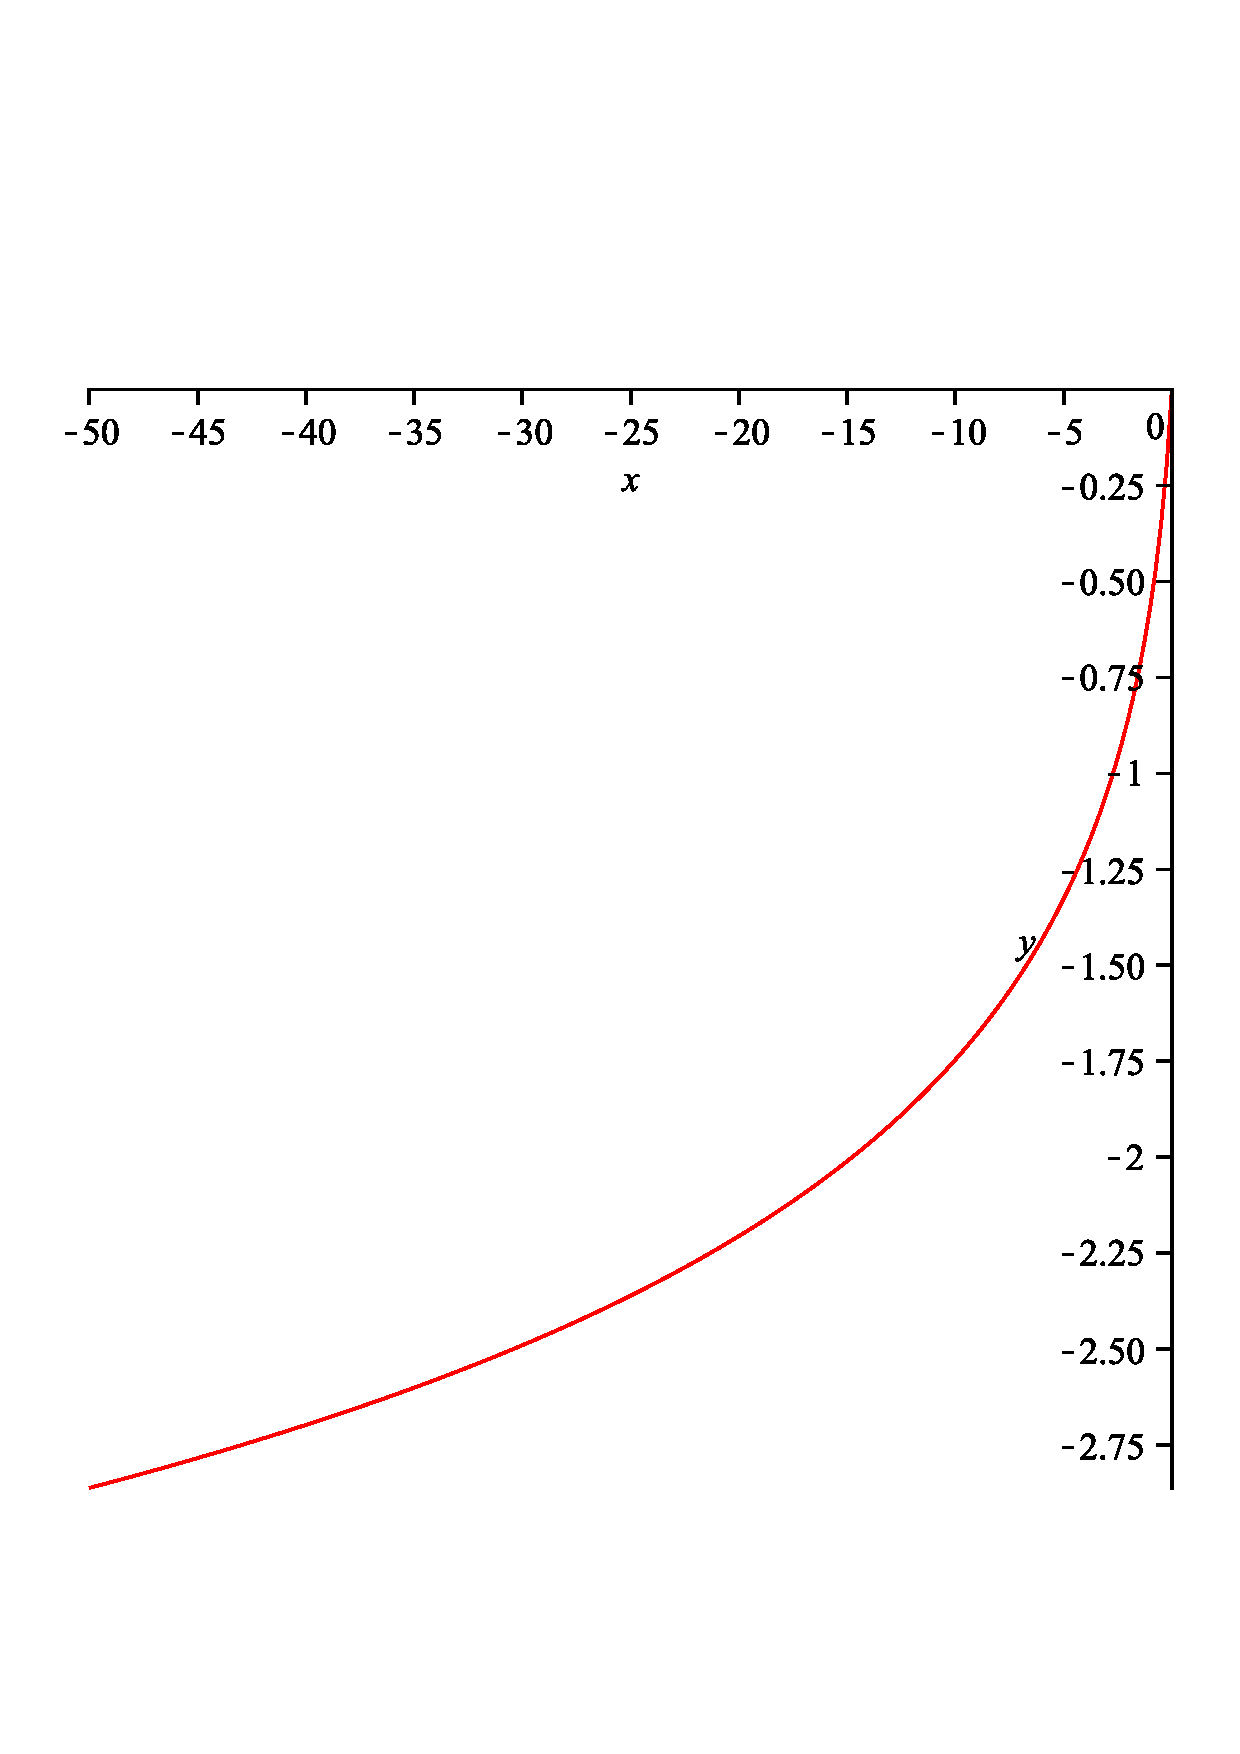
\includegraphics{ExpLinNeg}\\
  \caption{$y=\textcolor{red}{\expL_-(}x\textcolor{red}{)}$}\label{FigExpLinNeg}
\end{figure}

\newpage
\begin{figure}[!h]
  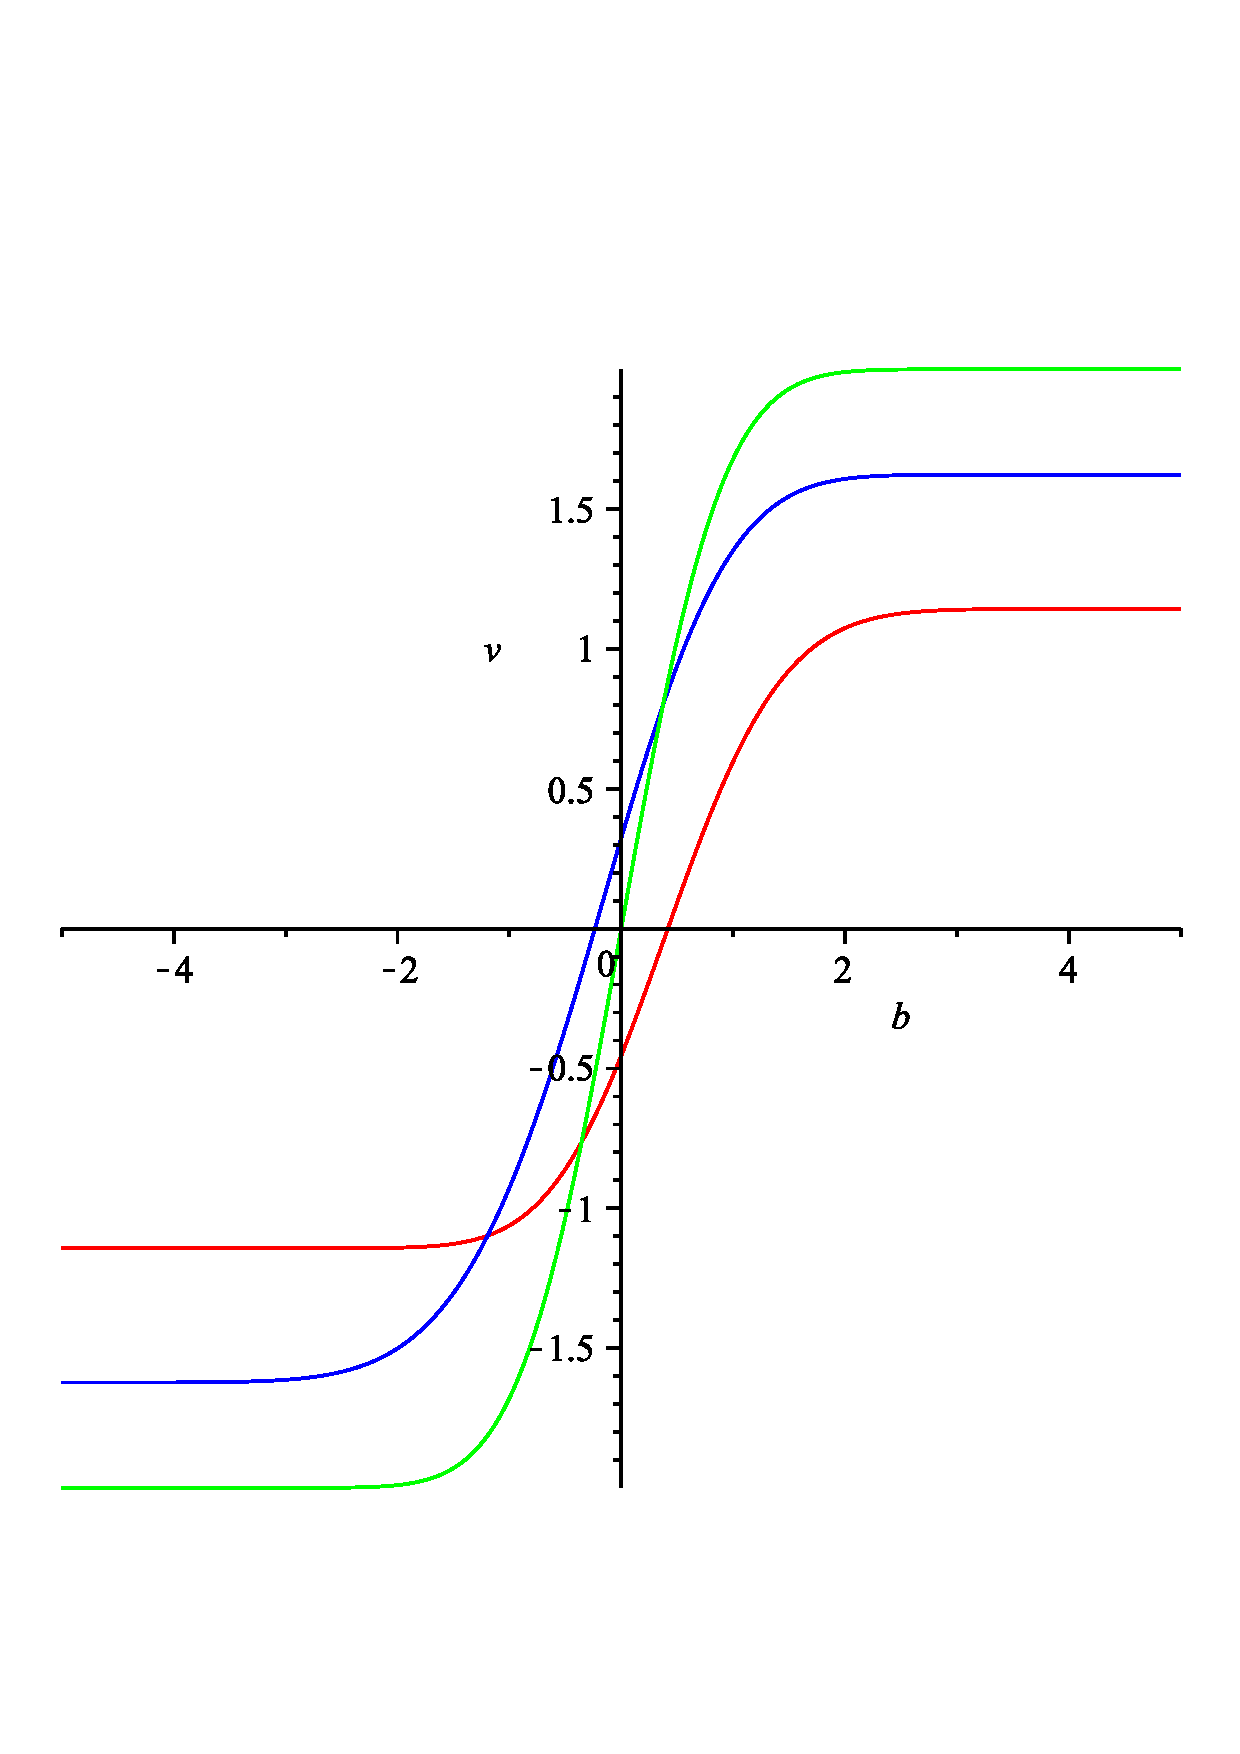
\includegraphics{ErfExpInt_b}\\
  \caption{$v=\textcolor{red}{\eeI(}0.89,\ b,\ 0.127\textcolor{red}{)},\;
              \textcolor{blue}{\eeI(}-1.13,\ b,\ 0.624\textcolor{blue}{)},\;
              \textcolor{green}{\eeI(}0.12,\ b,\ 2.35\textcolor{green}{)}
           $
          }\label{FigErfExpInt_b}
\end{figure}

\newpage
\begin{figure}[!h]
  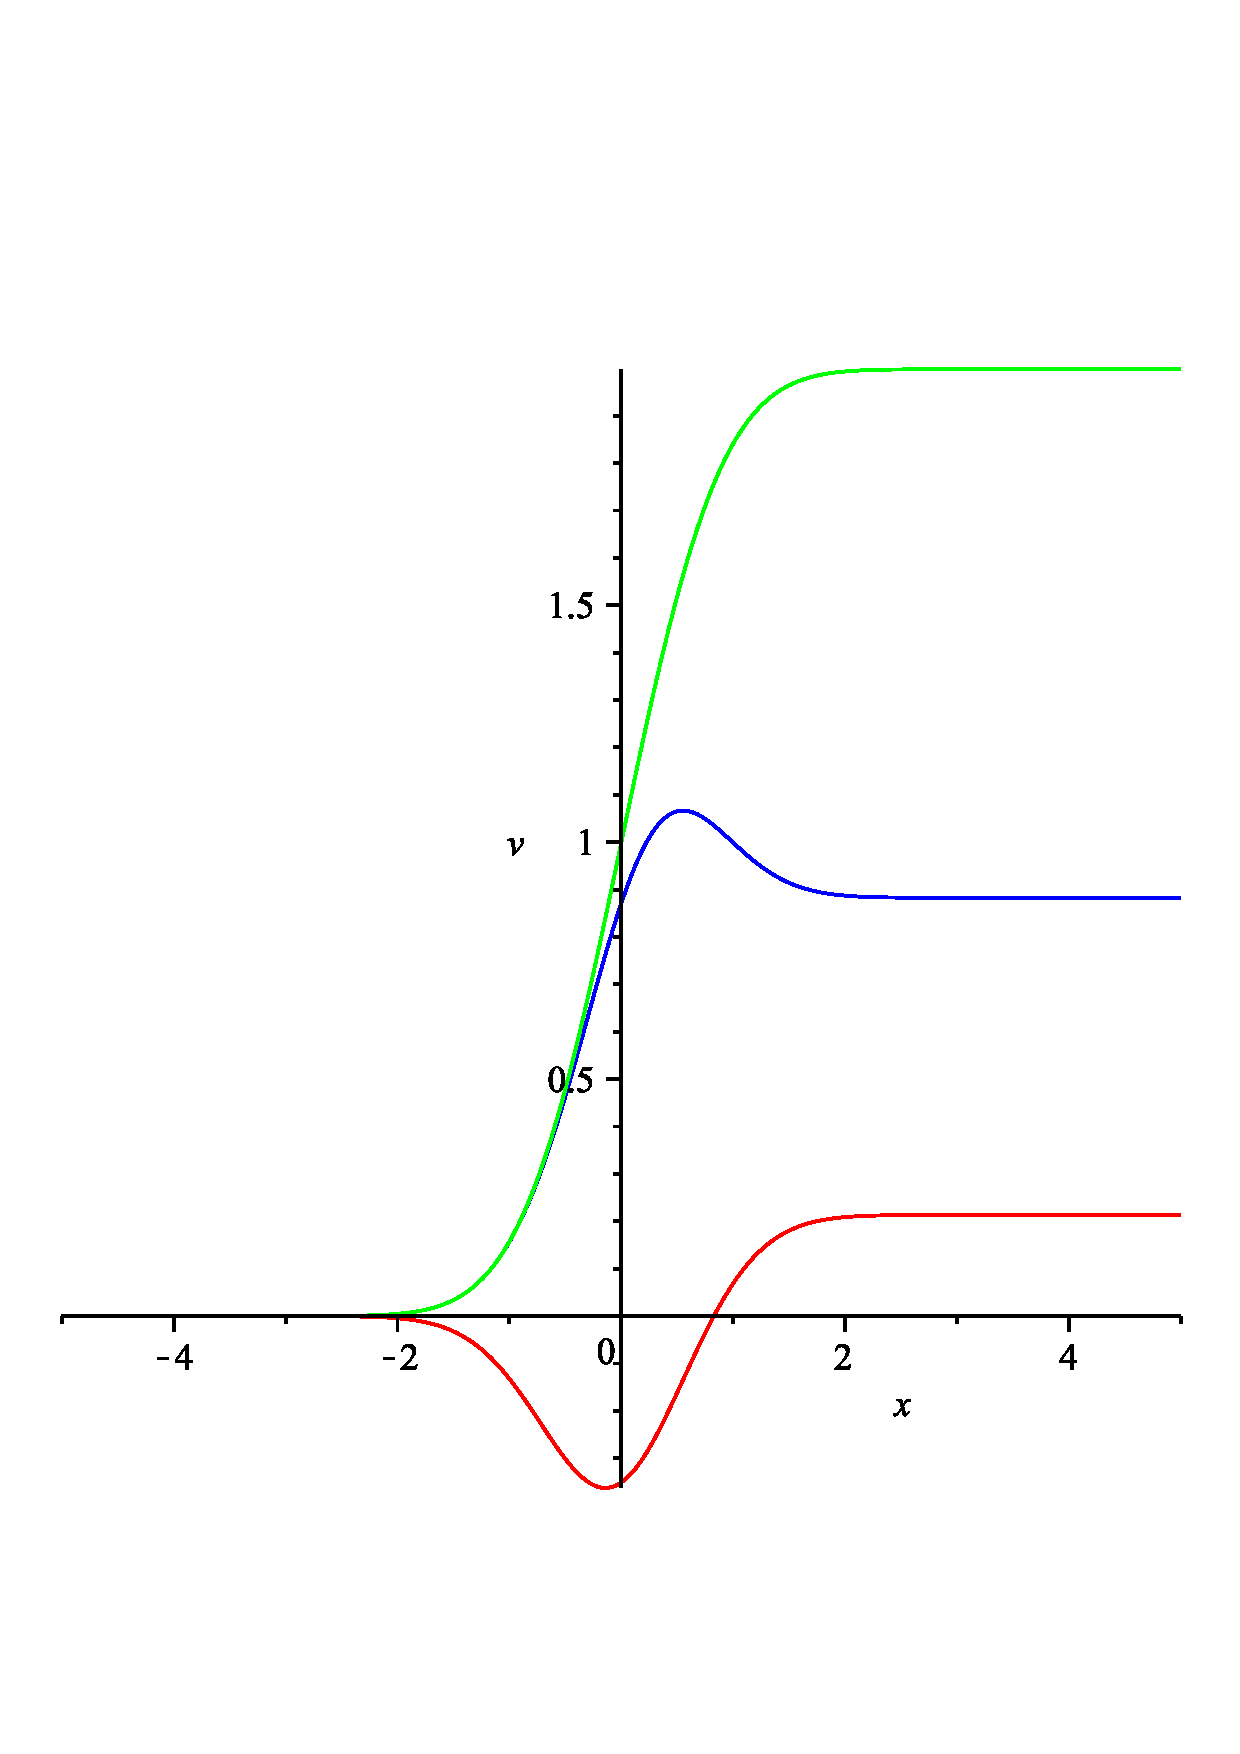
\includegraphics{ErfExpInt_x}\\
  \caption{$v=\textcolor{red}{\eeI(}0.89,\ 0.127,\ x\textcolor{red}{)},\;
              \textcolor{blue}{\eeI(}-1.13,\ 0.624,\ x\textcolor{blue}{)},\;
              \textcolor{green}{\eeI(}0.12,\ 2.35,\ x\textcolor{green}{)}
           $
          }\label{FigErfExpInt_x}
\end{figure}


\end{document} 